\documentclass[a4paper,11pt]{article}
\usepackage[T1]{fontenc}
\usepackage[utf8]{inputenc}
\usepackage{lmodern}
\usepackage{hyperref}
\usepackage{graphicx}
\usepackage{rotating}
\usepackage{listings}
\usepackage{color}

% Swedish
\usepackage[swedish]{babel}

% Table of contents depth 3 levels: A.B.C
\setcounter{tocdepth}{3}

\begin{document}

\title{{\huge Sommarstugekoll} \\
	Digital Konstruktion EDA234 \\ Grupp 2}
\author{Fredrik Brosser, Karl Buchka, Andreas Henriksson, Johan Wolgers \\ \\
   	Chalmers Tekniska Högskola \\ \\
	\begin{tabular}{l c r}
		\texttt{frebro} & \texttt{@} & \texttt{student.chalmers.se}\\
		\texttt{karlbu} & \texttt{@} & \texttt{student.chalmers.se}\\
		\texttt{henriksa} & \texttt{@} & \texttt{student.chalmers.se}\\
		\texttt{wolgers} & \texttt{@} & \texttt{student.chalmers.se}\\\\
	\end{tabular}
	}

\maketitle

\pagebreak

\tableofcontents

\pagebreak

\begin{center}
	{\noindent \bf Sammanfattning}
\end{center}

	Ett system för temperaturavläsning och relästyrning beskrivs genom denna rapport. Systemet är åtkomligt och styrbart via telefon genom DTMF (Dual Tone Multiple Frequency). Systemets funktion består i att informera användaren om aktuella temperaturer från två temperatursensorer samt ge användaren möjlighet att via telefon styra utgångarna (till/från) för exempelvis värmeelement eller belysning. Styrning och återkoppling utbytes genom en telefonlinje, POTS (Plain Old Telephone Service) med hjälp av DTMF.

En tänkt tillämpning för produkten:
\begin{list}{*}{}
\item Systemet inkopplas innan avfärd från sommarstugan och befinner sig i viloläge. 
\item Användaren kan då denne önskar ringa upp systemet som på anmodan returnerar temperatur från någon av temperaturgivarna.
\item Användaren kan sedan genom sin knapptelefon aktivera eller avaktivera någon av utgångarna för att på så sätt slå till värme, belysning eller vad som anslutits till funktionsutgångarna.
\end{list}

\begin{center}
	{\noindent \bf Abstract}
\end{center}

	The system described in this report is an automated domestic temperature control system, accessible and controllable via
	a standard telephone connection (DTMF). The main functionality of the system is informing the user of the current temperatures
	at the points of measurement, and also to give the user the ability to remotely control (simple on/off) a number of external
	functions. These functions could be, for example, heating systems, radiators or air conditioning. Information- and control data
	is exchanged via a standard, analog telephone connection, using DTMF: Dual Tone, Multiple Frequency.

	A specific, practical usage example is the concerned holiday home owner wanting to keep control of the heating in his summer house.
	Using Sommarstugekoll, one can keep the temperature at a reasonable level, avoiding for example pipes freezing, but at the same time
	keeping the total heating costs to a minimum. Sommarstugekoll solves this by offering users a neat and simple way to keep track
	of in- and outdoor temperatures - when the previously mentioned summer house owner wishes to make a visit, he simply dials the
	summer house telephone number giving it instructions to bring the temperature up to a comfortable level, all while he makes
	the drive up. Simple - smart - elegant - Sommarstugekoll is the domestic temperature automation assistant of the future!

\pagebreak

\section{Introduktion}

	Konstruktionsprojektet utförs inom kursen ``Digital Konstruktion, EDA234'' vid Chalmers Tekniska Högskola. Uppgiften består att inom gruppen om 4 personer konstruera och dokumentera
	ett digitalsystem utifrån en specifikation, med fokus låg på huvudfunktionalitet i det digitala området. Utvecklingen sker på ett färdigt utvecklingskort vilket sedan kompletteras med externa kretsar och programmeras för att nå kravspecefikationen. Logikkretsen som används är en Xilinx XC9572XL CPLD, och utveckligen sker i huvudsak med VHDL i Xilinx ISE-miljön samt i ModelSim för simuleringar. Rapporten är uppdelad i abstraktionslager med fördjupningar i de senare avsnitten. 

	En handhavandeinstruktion återfinns bifogad i \ref{sec:Användarmanual och Gränssnitt}.

\pagebreak

\section{Systembeskrivning och -specifikation}

	\subsection{Specifikation}

	Huvudfunktionen hos systemet är att användaren skall kunna ringa upp systemet och få inne- och utetemperaturen
	uppläst. Sedan skall användaren kunna kontrollera på/av-status för ett antal olika funktioner. Temperaturen
	läses av med hjälp av temperatursensorer och ges med en upplösning på +/- 0.5C i mätintervallet +/- 32.0C.
	Kommandon till funktionsstyrningen ges via att användaren trycker motsvarande knapp på sin telefonknappsats.
	Vidare finns även en fysisk, manuell knappsats på systemet för direkt styrning. Utöver att läsas upp i 
	telefonen visas den aktuella temperaturen (binärt) på en LED-Display. Funktionsstatus samt ON/OFF för systemet
	visas på lysdioder.

	\subsection{Uppdelning}

	Systemet består av ett antal delblock (moduler), och är skrivet för att vara så modulärt som möjligt.
	Nedan följer en sammanfattande tabell över de olika modulerna och deras funktioner. Varje modul är mer
	utförligt beskriven i sektionen {\it Block, Funktionalitet}. För en komplett överblick, se Blockschema. \\\\

	\begin{tabular}{l r}
		{\bf Modul} & {\bf Funktion}\\
	   	Styrenhet & Samordnar systemfunktioner\\
	  	Temperaturmodul & Initierar, läser och presenterar temperatur\\
	   	DTMF-modul & Tar emot DTMF-signaler från användaren\\
		Ljudmodul & Spelar upp ljud lagrade på extern minneskrets\\
		Knappsatsmodul & Hanterar knapptryckningar från användaren\\
		Funktionsmodul & Hanterar funktionerna och deras status\\\\
	\end{tabular}

	Systemet är uppdelat enligt dataväg-styrenhet-modellen, där designprincipen går ut på att skilja styrsignaler
	och dataflödeskontroll (Styrenheten) från själva datan som forslas genom systemet (Datavägen). Den data som
	skickas inom systemet är i första hand temperaturdata från temperaturmodulen till ljudmodulen, och ljud som
	lagras på den externa ljudlagringskretsen och hanteras av ljudmodulen. Detta flöde kontrolleras från styrenheten via
	enkla styrsignaler. Viss data, i form av indata från användargränssnitt och utdata till funktionsstatus, passerar
	dock genom styrenheten.

	\subsection{Översikt}

	Systemet bygger på DTMF-kommunikation (Dual Tone Multiple Frequency, Tonval). Telefonen skickar ut DTMF-signaler, som kan
	läsas och avkodas av DTMF-avkodarkretsen, MT8880. DTMF-signaler består av två toner som tillsammans unikt ger vilken
	siffra på telefonens knappsats som användaren tryckt på. Systemet börjar med att läsa upp ett antal ljudklipp med
	aktuella temperaturer, och erbjuder sedan användaren möjligheten till att styra de externa funktionerna.
	DTMF-Mottagaren avkodar signalerna och skickar in den resulterande
	datan till CPLD'n. Beroende på vilket kommando användaren gett beslutar CPLD'n vad som skall hända näst. Är kommandot ett
	funktionskommand (Funktion på eller av) så sätter CPLD'n statusen för den specifika funktionen till det önskade. 

	\subsection{Blockschema}

	Se figurer i Appendix ~\ref{fig:BlockDiagram1} och ~\ref{fig:BlockDiagram2}

	\begin{figure}[ht!]
	  \centering
	      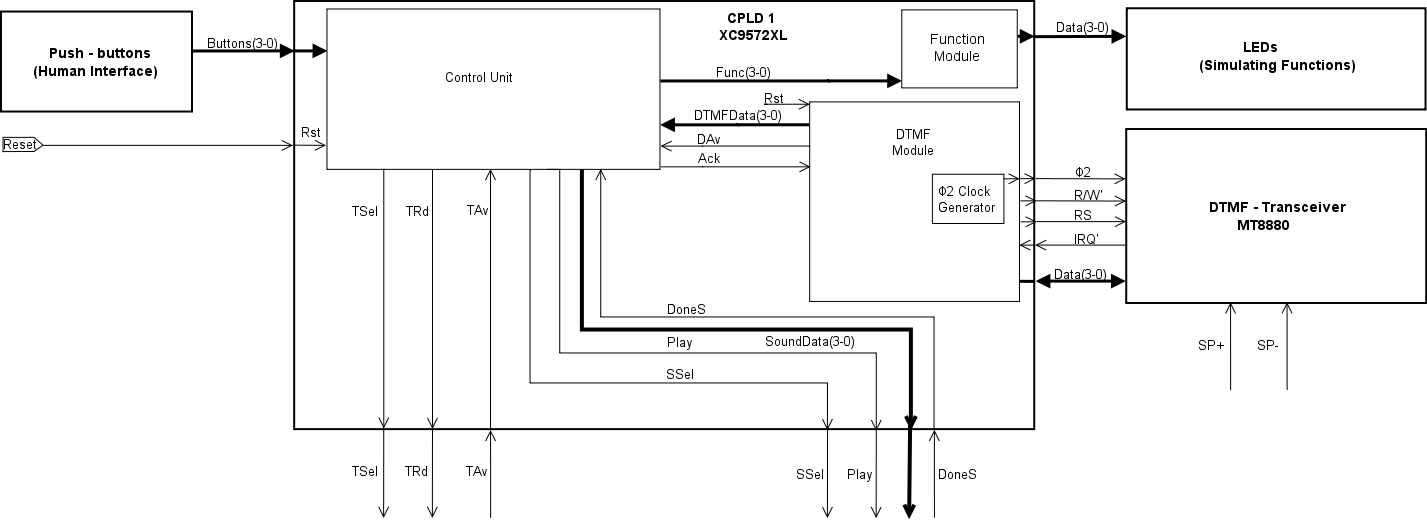
\includegraphics[scale=0.48, angle=90]{BlockDiagramCPLD1.png}
		\label{fig:BlockDiagram1}
	  	\caption{Blockschema (CPLD1)}
	\end{figure}

	\begin{figure}[ht!]
	  \centering
	      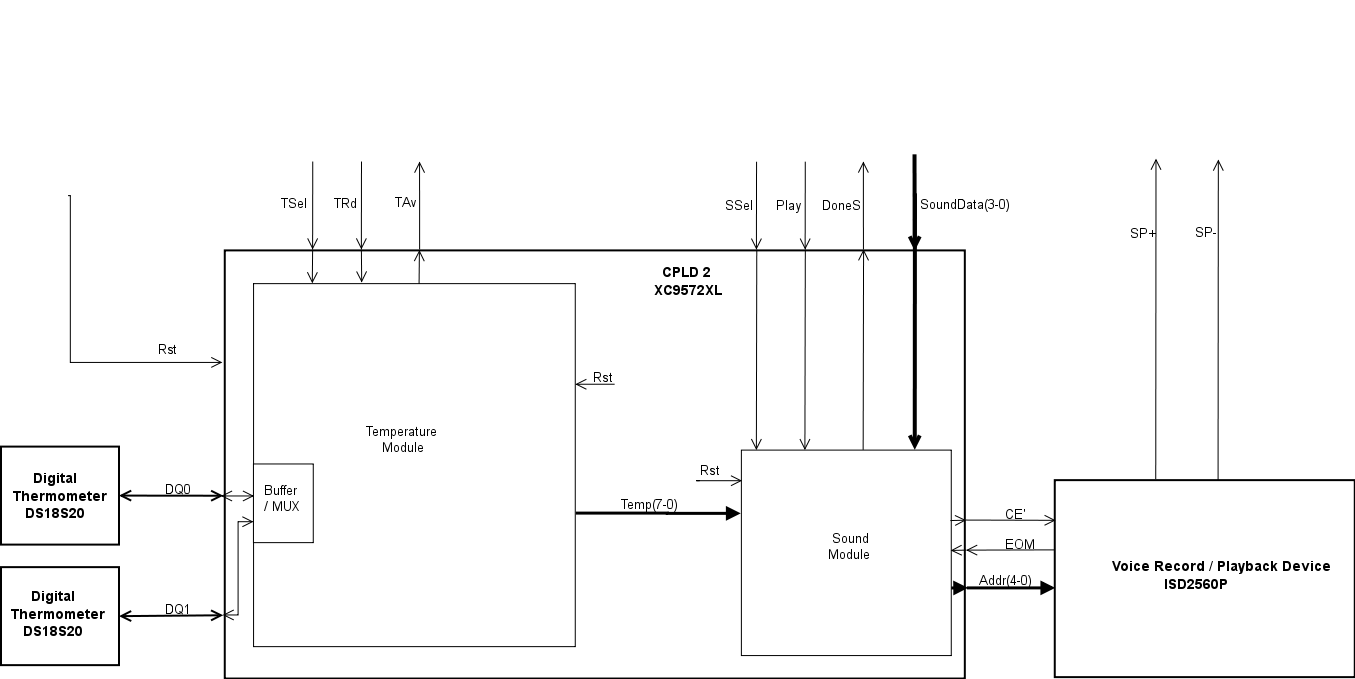
\includegraphics[scale=0.48, angle=90]{BlockDiagramCPLD2.png}
		\label{fig:BlockDiagram2}
	  	\caption{Blockschema (CPLD2)}
	\end{figure}

\section{Funktionsenheter}

	\subsection{Dataväg}

	\subsubsection{Modulbeskrivning}

	Den huvudsakliga datavägen är för temperaturdatan som skickas från Temperaturmodulen till Ljudmodulen,
	för vidare uppläsning via Ljudlagringskretsen, ISD2560P. Denna data skickas aldrig genom, men kontrolleras av,
	Styrenheten. Den rena datavägen i systemet är alltså här begränsad till CPLD2.

	\subsection{Styrenhet}

	\subsubsection{Modulbeskrivning}

	Styrenheten kontrollerar och ger styrsignaler för att överse de övriga systemdelarna. Syftet är att ge en
	lätt överblick över hela körningscykeln, där styrenheten har kontrollen över funktionerna via en rad styr-,
	available- och acknowledgesignaler. Styrenheten får även indata från knappsats och DTMF-mottagare via moduler
	som presenterar datan för styrenheten. Denna indata är skild från datavägen (temperaturinformation), och säger
	till styrenheten vad den ska göra härnäst, dvs. reagera på ett korrekt sätt på användarinput.

	\subsubsection{Uppbyggnad}

	Styrenheten är i sin tur modulärt uppbyggd, och har ett väl avgränsat interface mot varje annan delmodul, men
	fungerar samtidigt som en samordnare mellan de olika modulerna.

	\subsubsection{Tillståndsmaskin}

	För en ingående grafisk beskrivning av den bakomliggande tillståndsmaskinen, se sektionen om Tillståndmaskiner.

	\subsection{DTMF-Modul}
		
	\subsubsection{Modulbeskrivning}

	DTMF-Modulen i CPLD1 är ansvarig för att hantera kommunikation med Telefonen och därmed med användaren.
	När användaren trycker ner en knapp på telefonen så genereras en DTMF-signal som uppfattas och avkodas
	av DTMF-Modulen, som sedan presenterar den mottagna indatan för Styrenheten.
		
	\subsubsection{Initiering}

	DTMF-Modulen måste få en initieringspuls minst 100 ms efter spänningspåslag. Detta sker med hjälp av
	en extern tryckknapp, som beskrivet i användarmanualen. Under hela initieringen är Chip Select satt låg
	och RS0 satt hög. Initieringscykeln börjar med att DTMF-Modulen läser statusregistret på MT8880-kretsen enligt ett 		i databladet givet mönster, se även Sektionen {\it Hårdvara, MT8880C} för en komplett beskrivning.
	DTMF-Modulen är ansvarig för att ge ut rätt signalnivåer under initieringsfasen, vilket görs med hjälp av en
	tillståndsmaskin, som finns beskriven i sektionen {\it Tillståndsmaskiner}.
		
	\subsubsection{Läsning}

	Då den färdigställt initieringen går DTMF-Modulen över i ett läsläge, där den kontinuerligt lyssnar på och
	tolkar input från MT8880C-kretsen. När valid indata detekteras läses den och läggs ut på den interna
	DTMF-Databussen till styrenheten, varpå DTMF-Modulen signallerar "Data Valid" till Styrenheten. DTMF-Modulen
	väntar sedan på en Acknowledgementsignal (DAck) från Styrenheten, som bekräftelse på att denna sett och läst
	den valida datan. Läsningen sker genom att DTMF-Modulen läser Statusregistret hos MT8880C: om bit 2 är satt
	så har en ton tagits emot, och Receive-Data-Registret läses genom att sätta RS0 låg och R/W' hög (= Read).
	Sedan kan den mottagna datan, 4 bitar, läsas direkt från bussen.

	\subsection{Ljudmodul}

		\subsubsection{Modulbeskrivning}

		\subsubsection{Initiering}

		\subsubsection{Addressering och Uppspelning}

	\subsection{Temperaturmodul}

	\subsubsection{Modulbeskrivning}

	Temperaturmodulen i CPLD2 är ansvarig för att hantera seriekommunikationen med 
	DS18S20-temperatursensorerna, via entrådsbussarna, samt att ge ut de lästa temperaturerna
	i tecken-belopp-format till ljudmodulen, i syfte att låta den i sin tur spela upp de avlästa
	temperaturen för systemanvändaren. För en komplett beskrivning av temperatursensorkretsen, se sektionen Hårdvara.

	\subsubsection{1-Trådsbuss}

	Entrådsbussarna är anslutna till matningsspänning (+5V) genom ett pull-up-motstånd på 4.7kO, och
	ändarna av bussen är anslutna till mastern (CPLD) och sensorn (DS18S20), respektive. Då bussen
	befinner sig i viloläge dras den hög ("svag drivning") av pull-up-motståndet. När information
	skickas över bussen drar den kommunicerande (sändande) enheten bussen låg genom att driva den
	med en stark logisk nolla. Se figur ~\ref{fig:TempBus}

		\begin{figure}[ht!tb]
		  \centering
		      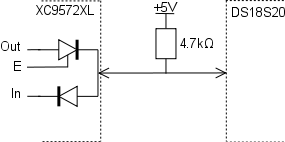
\includegraphics[scale=1, angle=0]{TempBus.png}
			\label{fig:TempBus}
		  	\caption{Uppkoppling, Entrådsbuss}
		\end{figure}

	\subsubsection{Läscykel}

	En läscykel består av fyra steg: Initialisering, Kommandon, Läsning och Viloläge.

	Se även figur ~\ref{fig:RCFlowChart} för en flödesdiagram-beskrivning av en komplett läscykel.

	Initialiseringen består i av att mastern driver bussen låg i 512 us, sedan släpper den.
	Temperatursensorn svarar med en närvaro-puls genom att driva bussen låg i 106 us, och därgenom bekräftar den sin 	 närvaro på bussen och sin operationella status.

	Då mastern detekterat närvaropulsen börjar den överföra ett ROM-kommando (Skip ROM, 0xCC), följt av en kort 		återhämtningslucka och sedan ett Funktions-kommando (Convert Temperature, 0x44), enligt läs-/skriv-luckemetoden som 		beskrivits ovan.
	Skip-ROM-kommandot används i det här systemet eftersom endast en temperatursensor används per entrådsbuss.
	Därmed finns inget behov av att kunna addressera specifika sensorer på bussen.
	Convert Temperature-kommandot säger till DS18S20-kretsen att börja konvertera temperaturen, och sedan spara den 
	lästa temperaturen i sitt interna minne för att sedan läsas av mastern.
	Under konverteringsperioden (upp till 750 ms) kan mastern polla temperatursensorns status genom att kontinuerligt
	sända förfrågningar genom att dra bussen låg i en kort period (4 us). Temperatursensorn svarar med en nolla
	sålänge den är upptagen med att konvertera temperatur, och sedan en etta såfort den är klar.
	Då mastern ser att temperatursensorn är klar, initiseras temperatursensorn om och ytterligare ett ROM-Funktions- 		kommandopar överförs. Dessa är 0xCC (Skip ROM) följt av 0xBE (Read Scratchpad), respektive.
	Idealt ska temperatursensorkretsen nu vara redo att överföra temperaturdata till mastern från sitt interna 
	9-bytesminne.
	Då den ges Read Scratchpad-kommandot börjar DS18S20 sända över innehållet i sitt minne över bussen.
	Mastern går då in i läsningsläget och börjar sampla datan på bussen genom att driva bussen låg, släppa den och sampla efter 4 us,
	allt enligt den metod som beskrivs ovan. Mastern samplar de första åtta bitarna data som sänds av DS18S20, sedan en ytterligare,
	nionde bit. Den sista biten utgör en tecken-bit, 0 för positiv temperatur och 1 för negativ. Då den nionde biten data lästs
	ger mastern på nytt en initieringspuls, som säger åt temperatursensorn att sluta sända data.
	Den nyligen lästa temperaturen placeras av temperaturmodulen i CPLD'n (på CPLD2) på den interna temperaturbussen, och
	TAv sätts till 1 för att indikera att det finns korrekt data på bussen, enligt vad som efterfrågades av styrenheten.

		\begin{figure}[ht!tb]
		  \centering
		      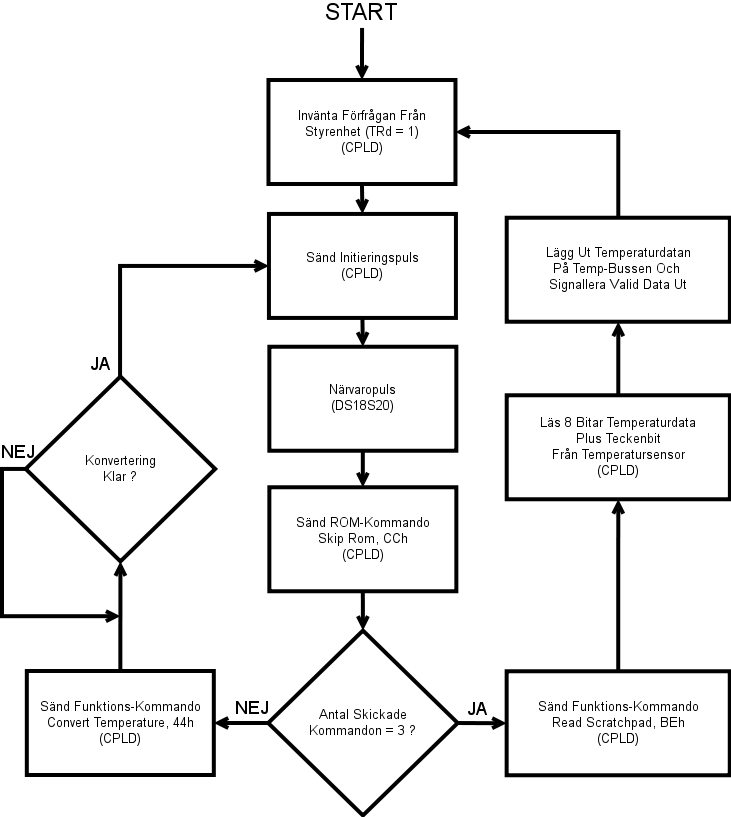
\includegraphics[scale=0.5, angle=0]{ReadCycleFlowChart.png}
			\label{fig:RCFlowChart}
		  	\caption{Högnivå-flödesdiagram för Temperaturläscykel}
		\end{figure}

	\subsubsection{Signaler}

		\begin{tabular}{l r}
			\\{\bf In} &  \\
			DQ0 & Kommunikationstråd till temperatursensor 0\\
			DQ1 & Kommunikationstråd till temperatursensor 1\\
			TRd & Styrsignal från styrenheten: Signalerar att läscykel ska inledas\\
			TSel & Styrsignal från styrenheten som väljer temperatursensor (0/1)\\\\
			{\bf Ut} &  \\
			TAv & Signal till styrenheten för att signalera att valid data finns på bussen\\
			Temp & Den interna temperaturdatabussen till ljudmodulen\\\\
		\end{tabular}

	\subsubsection{Uppbyggnad}

	Temperaturmodulen är baserad runt en tillståndsmaskin, understödd av en intern Buffer/MUX-modul samt 
	ett antal interna räknare för att generera de nödvändiga tidsfördröjningspulserna.

	\subsubsection{Buffer/MUX}

	Buffer/MUX-modulen är direkt ansluten till de två DS18S20-Temperatursensorerna som använder entrådsbusskommunikationen.
	Multiplexern (MUX) används för att välja mellan vilken av de två sensorerna (Sesnor 0 eller Sensor 1) som styrenheten
	vill kommunicera med, och använder signalen TSel.
	Buffern är en tri-state-buffer med en Enable-signal, E. När E är satt till 1 så kan mastern använda den av TSel valda
	entrådsbussen som en utgång för att överföra kommandon. När E är satt till 0 kan mastern läsa data från bussen.

	\subsubsection{Räknare}

	Internt använder temperaturmodulen ett antal olika räknare: \\
		\begin{tabular}{l c r}
			\\{\bf Namn} & {\bf Bitar} & {\bf Beskrivning}\\
			cntInt & 9 & Genererar timing-pulser\\
			ZC & 4 & Hanterar timing för skriv-luckor\\
			Progress & 2 & Anger aktuellt kommando (0-3)\\
			bitCnt & 8 & Anger aktuell bit för överföring/läsning\\\\
		\end{tabular}

	\subsubsection{Tillståndsmaskin}

	För en uttömmande grafisk beskrivning av den interna tillståndsmaskinen som används av temperaturmodulen,
	se sektionen om tillståndsmaskiner.

	\subsection{Extern funktionsstyrning}

\subsubsection{Modulbeskrivning}

Funktionsmodulen är mycket enkelt uppbyggd, den tar emot data från Styrenheten och skickar vidare 
uppdateringarna ut på de I/O-pinnar som används för funktionerna. Sammanfattat fungerar den som ett
mellansteg för att underlätta för styrenhetens funktionsstyrning, och kan vid behov byggas ut ytterligare
för att implementera andra funktioner i systemet.

	\subsection{Fysiskt användargränssnitt och Knappsats}

\subsubsection{Modulbeskrivning}

Se även grafisk beskrivning av användargränssnittet ~\ref{fig:UserInterface}
Systemet har, förutom DTMF-kontroll, även ett fysiskt gränssnitt med en knappsats samt en På/Av-Brytare för temperaturläsning.
Dessa rådata måste formateras, avkodas och presenteras för styrenheten. Detta är Knappsatsmodulens uppgift.

Om en knapp på knappsatsen trycks ned, skickas en availablesignal (DAv) från knappsatsen till knappsatsmodulen, som sedan
avkodar vilken knapp som tryckts ned, och presenterar detta för styrenheten genom att höja en KAv (Keyboard Available)-signal,
vilket indikerar valid data på knappsatsdatabussen, KData[3..0]. Genom att skicka en Acknowledgement-signal, KAck, bekräftar 
styrenheten att den sett och mottagit datan från knappsatsen.

\section{Hårdvara}

	\subsection{ISD2560P}

	\subsection{DS18S20}
	
		Den temperatursensor som används är Maxim DS18S20, som ger temperaturmodulen möjlighet att läsa av temperaturen
		med nio (9) bitars upplösning. Sensorerna som användas i detta system drivs av en extern spänningskälla på +5V,
		och kommunicerar seriellt över en entrådsbuss. Seriekommunikationen baserar på att bus-mastern initierar skriv-
		och läs-luckor. Varje sådan lucka är mellan 60 och 120 us lång. Temperatursensorn initieras genom att mastern
		driver bussen låg i åtminstone 480 us, vilket följs av att temperatursensorkretsen själv drar bussen låg i 60-240 us,
		efter en återhämtningslucka på minst 1 us. Efter initieringen väntar sensorkretsen på ett ROM-kommando från mastern,
		följt av ett Funktions-kommando. Varje sådant kommando är en byte lång, och skickas som LSB-först. Mastern skickar
		en logisk nolla genom att driva bussen låg under hela skrivluckan. En etta skickas genom att mastern driver bussen låg
		under en kort period, 1-15us, och sedan släpper bussen under resten av skrivluckans längd. Mellan varje skriv- eller läslucka
		måste det finnas en återhämtningsperiod på minst 1us.

		Då mastern är klar med att skicka över ROM- och Funktions-kommando, kan (beroende på vilka kommandon som sändes) DS18S20-kretsen
		svara med aktuell data. På samma sätt som ovan måste mastern här initiera en läs-lucka genom att driva bussen låg i 1-8us, och
		sedan släppa den (högimpediv). DS18S20-kretsen svarar på den allokerade läs-luckan genom att antingen hålla bussen låg för att
		överföra en nolla, eller genom att låta bussen dras hög av pull-up-motståndet för en etta. Under den här tiden (upp till 15 us
		efter att ha släppt bussen) kan mastern sampla bussen för att läsa av vad DS18S20-kretsen skickat. All data som skickas från
		temperatursensorn skickas som LSB-först, och i 2-komplementsform.\\

	\subsection{MT8880C}
	
		Avkodning av uppringandes DTMF-signaler avkodas med hjälp av MT8880C från Mittel. 
		Telefonsignalen kopplas direkt in till DTMF-överföraren enligt specifikation för standarsuppkoppling i datablad. Endast avkodningsfunktionen på 		kretsen används. Databuss, R/W-signal, IRQ och $\Phi$2 är anslutna till kontrollenheten. 
		CS (Chip Select) är satt konstant låg då denna krets använder bussen exklusivt. 
Före initiering skickas manuellt en initieringspuls till kretsen minst 100ms efter spänningspåslag. Sedan följer
en initieringscykel enligt nedan:\\

	{\bf Initiering}

	\begin{tabular}{l c c c r}
		\\{\bf Beskrivning} & {\bf CS'} & {\bf RS0} & {\bf R/W'} & {\bf Data[3..0]}\\
		Läs Statusregister 	& 0 & 1 & 1 & 0000\\
		Skriv till Kontrollreg. & 0 & 1 & 0 & 0000\\
		Skriv till Kontrollreg. & 0 & 1 & 0 & 0000\\
		Skriv till Kontrollreg. & 0 & 1 & 0 & 1000\\
		Skriv till Kontrollreg. & 0 & 1 & 0 & 0000\\
		Läs Statusregister 	& 0 & 1 & 1 & 0000\\\\
	\end{tabular}
	
	Efter initiering är kretsen klar att avkoda och ge ut DTMF-signaler. Polling av DTMF-data sker genom
	att läsa av statusregistret, där anges om en DTMF-ton tagits emot.

\section{Tillståndsmaskiner}
		\subsection{Styrenhet}
		\subsection{Temperaturmodul}
			Se state-machine-diagram: ~\ref{fig:TempSM} och förklaring ~\ref{fig:SMExp}\\
			{\bf Reset:} Alla signaler och räknare återställs till sina grundvärden.\\
			{\bf Grundvärden:} Utgångspunkten är att alla signaler behåller sina gamla värden om inget annat anges.\\
			\begin{tabular}{l}
				\\{\bf Viloläge (Tillstånd 0):}\\
				0: Viloläge och återställningspunkt. Inväntar TRd = 1 från Styrenheten\\
				{\bf Initialisering (Tillstånd 1-3):}\\
				1: Fördröjningstillstånd, väntar på puls på DelayLong (512 us)\\
				2: Mastern driver bussen låg i 512 us och sätter datavärdet till 0xCC (Skip ROM)\\
				3: Mastern släpper bussen, DS18S20 skickar närvaropuls\\
				{\bf Kommandoöverföring (Tillstånd 4-8):}\\
				4: Förberedelsetillstånd före sändning\\
				5: Huvudsändningstillståndet, mastern sänder bit enligt aktuellt räknarvärde\\
				6: Mellanbittillstånd, återhämtningstillständ. Fortsätter om fler bitar ska skickas\\
				7: Avgör om DS18S20 är upptagen med att konvertera temperaturen. Om så, vänta tills klar\\
				8: Vägskälstillstånd. Om vi har fler kommandon att skicka, gå tillbaka, annars börja läsa\\
				{\bf Läsning (Tillstånd 9-15):}\\
				9:  Förberedelsetillstånd före läsning\\
				10: Mastern initierar en läslucka genom att dra bussen låg i 4 us\\
				11: Mastern väntar ytterligare 4 us för att pull-up-motståndet ska få verka\\
				12: Mastern samplar bussen. Om DS18S20 skickar en nolla hålls bussen låg, annars inte\\
				13: Återhämtningstillstånd mellan samplingar\\
				14: Vägskälstillstånd. Om vi har fler bitar att läsa, gå tillbaka, annars gå vidare\\
				15: Läsning klar, lägg ut temperatur på buss och signallera valid data. Gå tillbaka till 0\\
			\end{tabular}

	\begin{figure}[ht!tb]
	  \centering
	      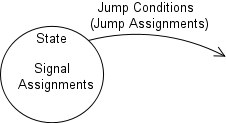
\includegraphics[scale=0.5, angle=0]{StateMachineExplained.png}
		\label{fig:SMExp}
	  	\caption{Förklaring till State Machine-diagram}
	\end{figure}

	\begin{figure}[ht!tb]
	  \centering
	      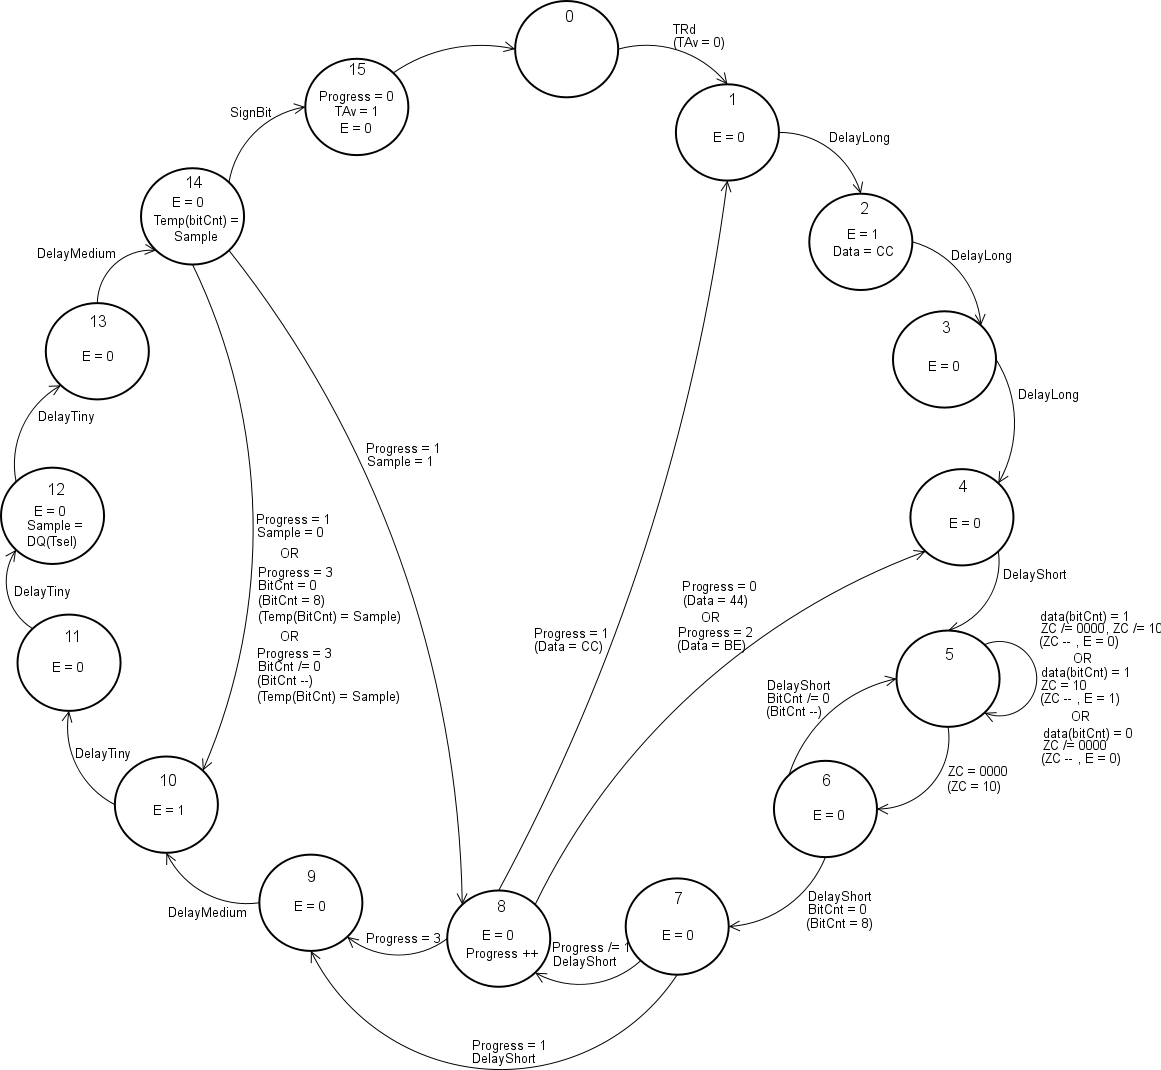
\includegraphics[scale=0.4, angle=0]{TempStateMachineDiagram.png}
		\label{fig:TempSM}
	  	\caption{Detaljerat State Machine-diagram för Temperaturläscykel}
	\end{figure}

		\subsection{DTMF-Modul}
		\subsection{Ljudmodul}

\section{Felanalys}

\subsection{Temperaturmätfel}

Då systemet hanterar avläsning av temperaturer och endast klarar ett begränsat temperaturintevall
görs här en felanalys (mätfel). För de tillämpningsområden systemet är konstruerat för (Hemanvändare) 
är mätfelen dock för små för att ha betydelse.

Temperatursensorerna arbetar med en temperaturupplösning på 0.5C, och här fås alltså därför en oexakthet.
Enligt temperatursensorns datablad gäller exaktheten på +/- 0.5C i intervallet -10C till +85C.
Systemet arbetar med ett temperaturspann på +/- 32C, allt utanför intervallet representeras som maxtemperaturen.

Testning av temperaturavläsningen har gjorts under utvecklingsperioden genom att värma och kyla temperatursensorerna,
och sensorerna visade de väntade resultaten, då jämförelser gjordes för inom- och utomhustemperatur kontrollerat med
en vanlig, kommersiell fönstertermometer med samma upplösning. Slutsatsen från jämförelserna blir att de två 
termometrarna följer varandra bra, och det går inte att avgöra vilken som är mer exakt. För vanlig hemanvändning
är båda fullt tillräckliga.

Jämförelserna och resultaten presenteras i en tabell nedan: 

	\begin{tabular}{l c r}
		\\{\bf DS18S20} & {\bf Fönstertermometer} & {\bf Differens [C]}\\
		4.5 & 5 & -0.5\\		
		11 & 9 & 2\\		
		18 & 18 & 0\\
		20 & 20 & 0\\	
		22 & 22 & 0\\
		25 & 26 & 0\\		
		36.5 & 37 & -0.5\\
		70.5 & 73 & -2.5 \\\\
	\end{tabular}

\pagebreak
{\bf \huge Appendix}

	\appendix
	\section{Användarmanual och Gränssnitt}

	För att använda systemet, koppla in det till en spänningskälla (+5V) och till en telefonlinje (RJ11).
	När systemet är startat ska det startas om (Röd tryckknapp) och sedan initieras (Svart tryckknapp).
	Efter detta är systemet redo att användas, och kommandon kan ges via telefon eller manuell knappsats.
	När som helst kan systemet startas om helt genom att igen trycka på den röda tryckknappen.
	Då systemet blir uppringt läses temperaturen upp, sedan kan kommandon ges från användaren enligt nedan:\\

	\begin{table}[ht]
		\begin{minipage}[b]{0.5\linewidth}\centering
			{\bf Knappsats}\\
			\begin{tabular}{l c r}
				\\{\bf Knapp} & {\bf Funktion}\\
				1 & Funktion 1 PÅ\\		
				2 & Funktion 2 PÅ\\		
				3 & Funktion 3 PÅ\\
				4 & Funktion 1 AV\\	
				5 & Funktion 2 AV\\
				6 & Funktion 3 AV\\		
				A & Visa Innetemperatur\\
				B & Visa Utetemperatur \\\\
			\end{tabular}
	 	\end{minipage}
	 	\hspace{0.5cm}
	 	\begin{minipage}[b]{0.5\linewidth}
			\centering
			{\bf Telefon}\\
			\begin{tabular}{l c r}
				\\{\bf Knapp} & {\bf Funktion}\\
				1 & Funktion 1 PÅ\\		
				2 & Funktion 2 PÅ\\		
				3 & Funktion 3 PÅ\\
				4 & Funktion 1 AV\\	
				5 & Funktion 2 AV\\
				6 & Funktion 3 AV\\
				9 & Visa Innetemperatur\\
				0 & Visa Utetemperatur \\\\
			\end{tabular}
	 	\end{minipage}
	\end{table}

		\begin{figure}[ht!]
		  \centering
		      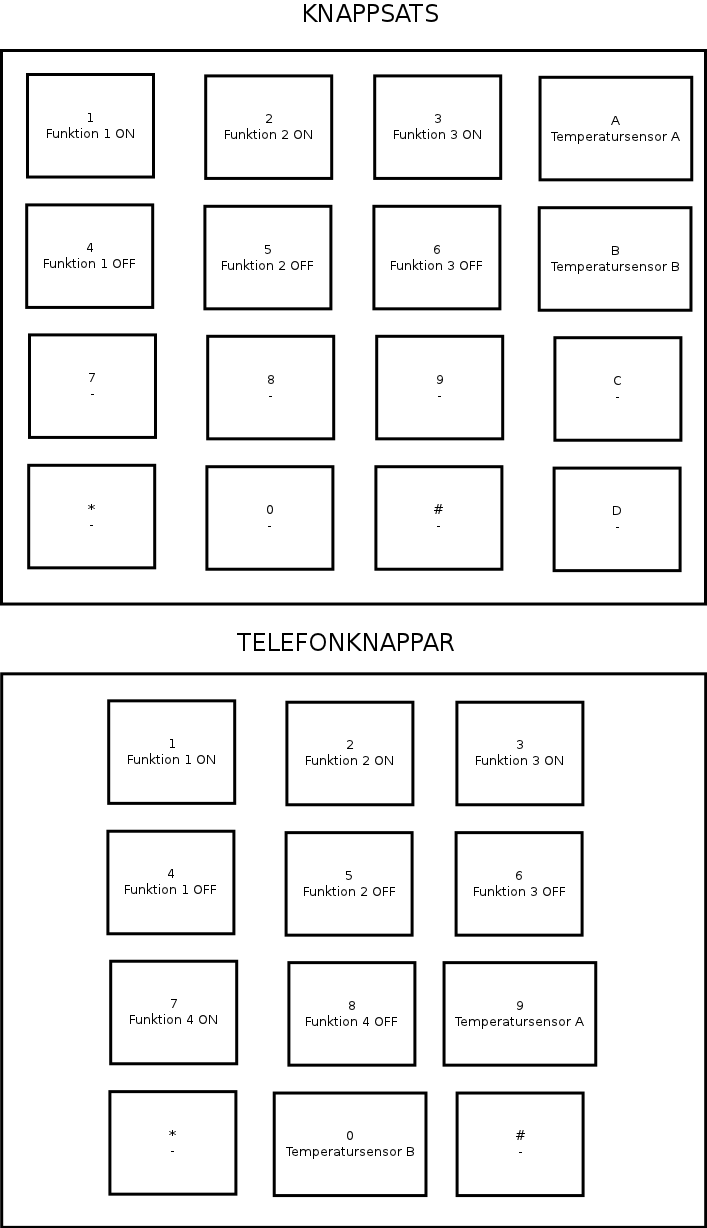
\includegraphics[scale=0.48, angle=0]{UserInterface.png}
			\label{fig:UserInterface}
		  	\caption{Knapplayout, Knappsats resp. Telefon}
		\end{figure}

	\section{Komponentlista}

	\section{Kretsschema}

		\begin{tabular}{ l r}
		   	Matningsspänning & +5V\\
		   	Strömförbrukning & ~80mA\\
		   	Temperaturmätspann & +/- 31.5 C\\
			Temperaturupplösning & 0.5 C\\	
		\end{tabular}

	\section{Pin-Layout}

		\begin{figure}[ht!]
		  \centering
		      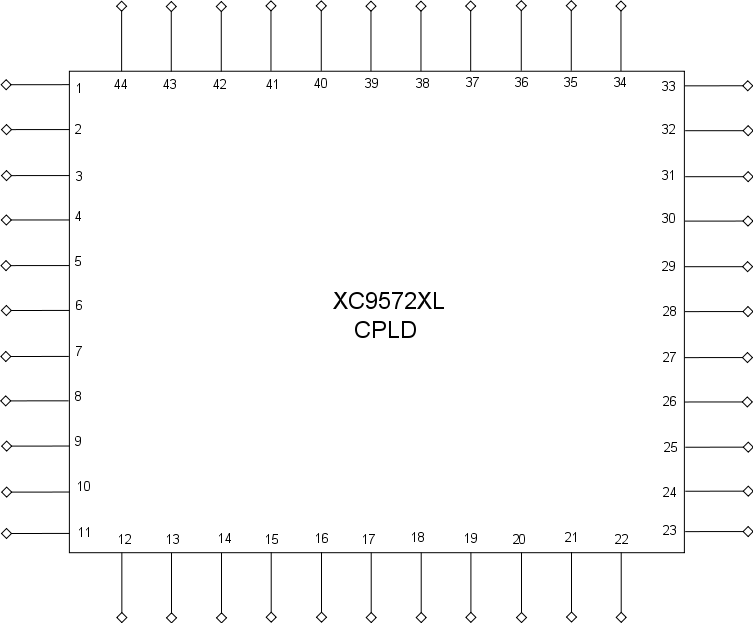
\includegraphics[scale=0.48, angle=0]{PinDiagram.png}
			\label{fig:Pin1}
		  	\caption{Pin-Konfiguration (CPLD1)}
		\end{figure}

		\begin{figure}[ht!]
		  \centering
		      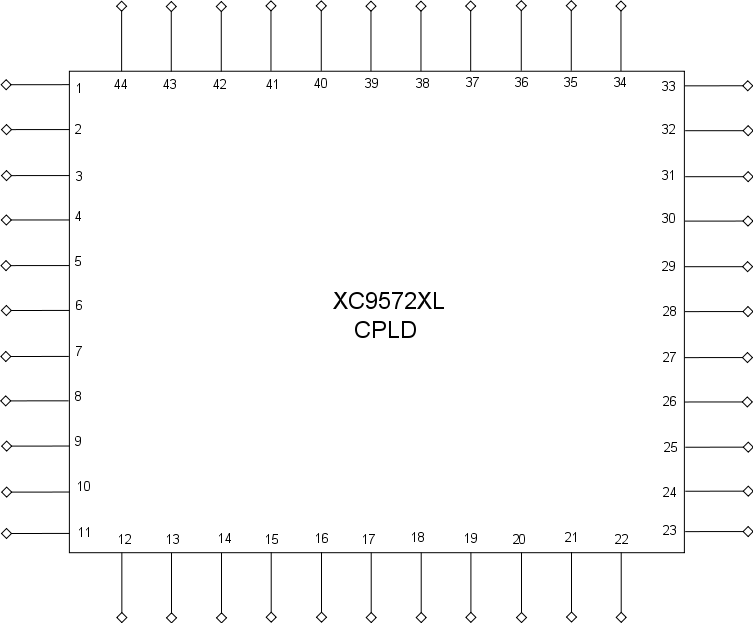
\includegraphics[scale=0.48, angle=0]{PinDiagram.png}
			\label{fig:Pin1}
		  	\caption{Pin-Konfiguration (CPLD2)}
		\end{figure}

	\section{Kretskortslayout}
	
	\section{Timingdiagram}

		\begin{figure}[ht!tb]
		  \centering
		      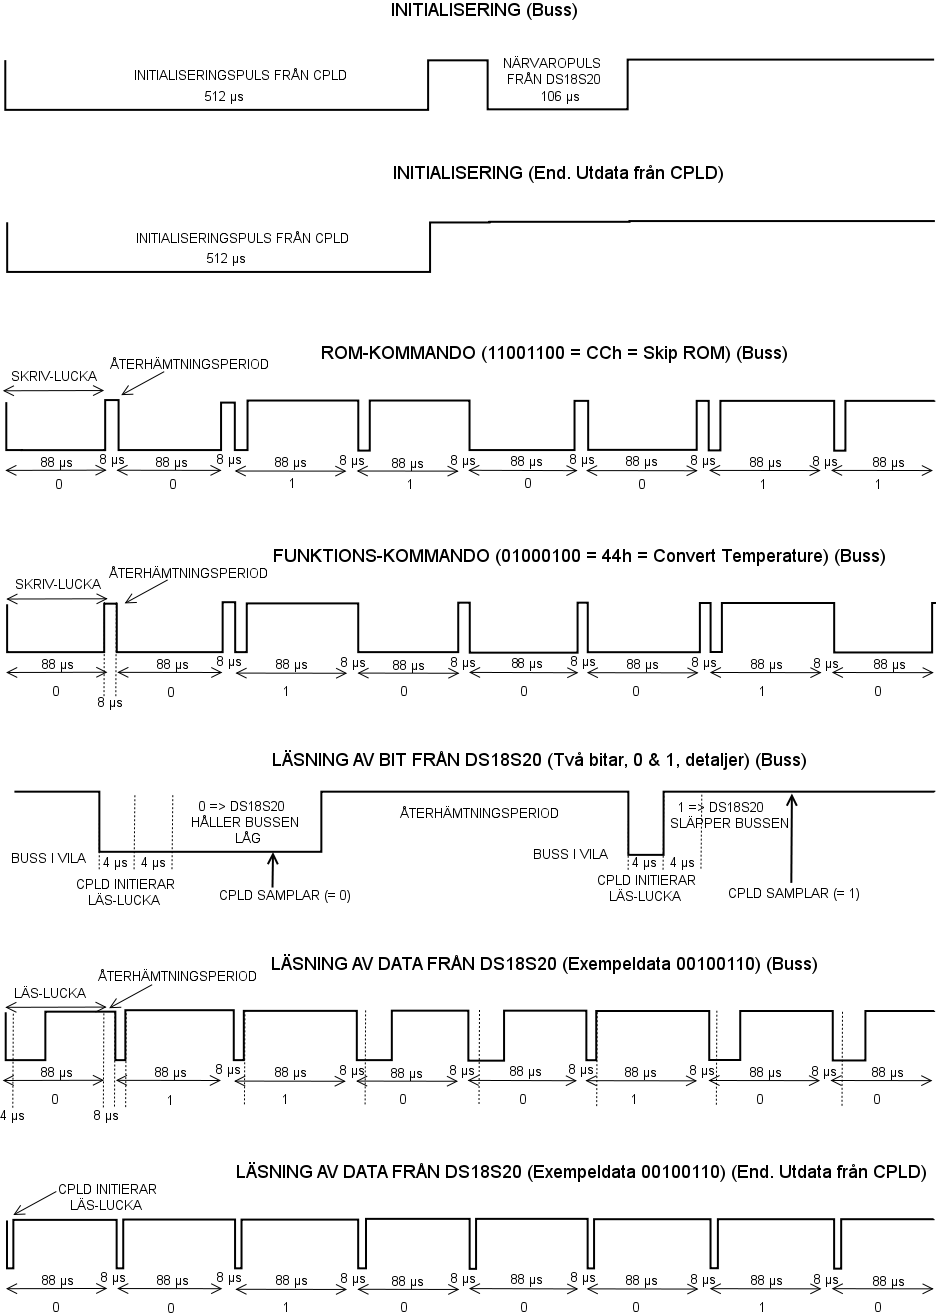
\includegraphics[scale=0.5, angle=0]{TempTiming.png}
			\label{fig:TempTiming}
		  	\caption{Timingdiagram för Temperaturmodulen}
		\end{figure}

	\section{Signallista}
	\begin{tabular}{l c c r}
		\\{\bf Signal} & {\bf Från} & {\bf Till} & {\bf Beskr.}\\ \\
		clk & Extern & Allt & Global Klocksignal\\
		rst & Extern & Allt & Global Resetsignal\\
		Buttons[3..0] & Knappsats & Knappsatsmodul & Indatavektor\\
		KBDav & Knappsats & Knappsatsmodul & Availablesignal\\
		FuncData[3..0] & Funktionsmodul & FunktionsLEDs & Funktionsstyrning\\
		DTMFData[3..0] & DTMF-Modul & MT8880 & Databuss till MT8880 (bidir.)\\
		Phi2 & DTMF-Modul & MT8880 & Klocksignal till MT8880\\
		R/W & DTMF-Modul & MT8880 & Read/Write till MT8880\\
		RS0 & DTMF-Modul & MT8880 & Intieringssignal till MT8880\\
		IRQ & MT8880 & DTMF-Modul & Interruptsignal från MT8880\\

		KData[3..0] & Knappsatsmodul & Styrenhet & Data från knappsatsmodul\\
		KAv & Knappsatsmodul & Styrenhet & Availablesignal från knappsatsmodul\\
		KAck & Styrenhet & Knappsatsmodul & Ack. till knappsatsmodul\\

		TSel & Styrenhet & Temperaturmodul & Sensorselectsignal\\
		TRd & Styrenhet & Temperaturmodul & Read-signal (starta läsning)\\
		TAv & Temperaturmodul & Styrenhet & Availablesignal, valid data\\

		SData[3..0] & Styrenhet & Ljudmodul & Ljudadressbuss\\
		SSel & Styrenhet & Ljudmodul & Selectsignal för temperatur/ljud\\
		SPlay & Styrenhet & Ljudmodul & Play-signal (spela ljud)\\
		SDone & Ljudmodul & Styrenhet & Signallerar uppspelning färdig\\

		DData[3..0] & DTMF-Modul & Styrenhet & DTMF-Databuss\\
		DAv & DTMF-Modul & Styrenhet & Availablesignal från DTMF-Modul\\
		DAck & Styrenhet & DTMF-Modul & Acknowledgement från Styrenhet\\

		FData[3..0] & Styrenhet & Funktionsmodul & Funktionsstatusbuss\\

		SP+ & ISD250P & MT8880 & Analog ljudsignal (+)\\
		SP- & ISD250P & MT8880 & Analog ljudsignal (-)\\

		DQ0 & Temperaturmodul & DS18S20 & Seriell 1-trådsbuss (bidir.)\\
		DQ1 & Temperaturmodul & DS18S20 & Seriell 1-trådsbuss (bidir.)\\

		Temp[7..0] & Temperaturmodul & Ljudmodul & Temperaturdatabuss\\

		Addr[4..0] & Ljudmodul & ISD2560P & Adressbuss till ISD2560P\\
		CE & Ljudmodul & ISD2560P & Chip-Enable från ljudmodul\\
		EOM & IDS2560P & Ljudmodul & End-Of-Message från ISD2560P\\\\
	\end{tabular}

	\section{Arbetsfördelning}

	\begin{tabular}{l c r}
		\\{\bf Namn} & {\bf Moduler / Ansvar} & {\bf Övrigt}\\
		Fredrik Brosser 	& ?? 	& ??\\
		Karl Buchka 		& ?? 	& ??\\
		Andreas Henriksson 	& ?? 	& ??\\
		Johan Wolgers 		& ??	& ??\\\\
	\end{tabular}

	\section{Programlistningar}
	
\end{document}
